\apendice{Plan de Proyecto Software}

\section{Introducción}

Vamos a ver cómo ha ido evolucionando el proyecto durante su realización, así como un estudio de viabilidad donde podemos ver si podemos llevarlo a cabo en el futuro.\cite{wiki:latex}

\section{Planificación temporal}
El proyecto se ha llevado a cabo utilizando metodologías ágiles, más concretamente SCRUM, realizando un numero de reuniones donde concretábamos los objetivos que íbamos a llevar acabo en cada sprint, no solo nos comunicábamos en estas reuniones, también utilizábamos el gestor de proyectos, Trello para resolver aquellas dudas que iban surgiendo durante la realización del sprint, una vez se acababa en el sprint en la reunión observábamos el trabajo realizado. Tanto en Trello como en GitHub podemos ver como se han ido desarrollando cada uno de los objetivos de los sprints.

\subsection{Sprint 1 (20/09/2016 – 04/10/2016)}
Es una toma de contacto con la gran cantidad de herramientas con las que vamos a trabajar. Lo primero y fundamental es la creación de una máquina virtual Ubuntu 14.04, sobre ella se va a instalar un servidor Apache, se va a seguir un tutorial que ha sido cedido por el tutor.
Tras analizar algunas herramientas de gestión de proyectos como Git, Bitbucket o GitHub, se decide trabajar con GitHub como gestor de versiones y con Trello como gestor de proyectos
Tras ello vamos a montar Drupal sobre el servidor Apache, durante la instalación de Drupal se han ido encontrado algunos problemas para enlazarlo correctamente con la base de datos que se ha creado durante la instalación de Apache.
Por último se empieza a investigar sobre el scraping y se crea un sencillo script con el que extraer algún dato.

\subsection{Sprint 2 (04/10/2016 – 21/10/2016)}
Lo primero es crear una estructura en la base de datos en la cual poder almacenar la información, que vamos a ir recopilando mediante los algoritmos de web scraping.
El primer algoritmo de scraping que vamos a crear es el que extraiga los resultados de los partidos y con ello todas las estadísticas. Es importante la selección de la página web sobre la que realizar el scraping ya que se necesitan una uniformidad en la URL. La primera página web que elegimos es la de Marca.com ya que la URL de los partidos es válida, el problema surge al extraer varios partidos ya que en algunos partidos directamente no hay estadísticas. Tras una larga búsqueda se encuentra otra página web, resultados-futbol en ella no nos encontramos con los problemas de Marca y la URL es válida.
Todos los datos que extraemos mediante el algoritmo de scraping hay que cargarlos en la base de datos, esto lo vamos a hacer utilizando una sintaxis de PHP especial para el acceso a MySQL a través de PHP. Inicialmente está habiendo muchos problemas para la utilización de algunas funciones de carga de datos.
Finalmente, se intentan añadir algunos temas a Drupal como por ejemplo el de Trello para poder trabajar driectamente sobre Drupal. Pero nos encontramos con un error de autentificación, que indagando por foros vemos que no tiene solución por lo cual descartamos estos y trabajamos con Trello independientemente desde el navegador.

\subsection{Sprint 3 (21/10/2016 – 08/11/2016)}
En este sprint tenemos que implementar el algoritmo de backpropagation, esto en un principio es un problema ya que mi conocimiento de PHP no es demasiado grande y el tiempo que se va a tardar en llevarlo a cabo puede extenderse. Valoramos diferentes algoritmos que vamos encontrando por internet, para tomarlos como base para la creación de nuestro algoritmo, finalmente nos quedamos con uno en Python y procedemos a su traducción a PHP, resulta costosa dado que este algoritmo en Python tiene clases y es así como lo vamos implementando  en PHP.
Creamos un algoritmo de scraping que extrae, de la misma página utilizada anteriormente para la extracción de resultados, las cuotas de las casas de apuestas, lo óptimo es la ejecución de este scrpit con la menor anterioridad a la jornada, ya que no todas las cuotas se encuentran en cualquier momento de la semana y estas van variando.

\subsection{Sprint 4 (08/11/2016 – 15/11/2016)}
Dado que el algoritmo no ha sido terminado correctamente decidimos prolongar su implementación a este sprint y tratamos de ver su respuesta ante una base de datos sencilla como Iris y más adelante probarle con otras bases de datos como balance, pima y wine. Tras varios ajustes en el código conseguimos una buena ejecución  con Iris.
Para ir preparando la entrada de datos a la red neuronal del algoritmo de backpropagation, se lleva a cabo un script que calcule las rachas de los equipos, además se realiza un tercer algoritmo de scraping para la recolección de los datos de cada equipo en la clasificación, este cambio conlleva un cambio en la base de datos.
Creamos las instancias para darlas de entrada en el algoritmo de backpropagation pero aún hay que hacer algunos ajustes ya que los datos no son del todo correctos.

\subsection{Sprint 5 (15/11/2016 – 23/11/2016)}
Lo primero en este Sprint es terminar las instancias que vamos a insertar en el algoritmo de backpropagation, en el anterior sprint se cargó la clasificación del equipo y la idea en un primer momento era hacer un update por cada jornada, en vez de esto vamos a cargar las clasificación de cada equipo en cada jornada, las rachas y la clasificación se unirán en la base de datos, teniendo la información de cada equipo en cada una de las jornadas.
Tras varias semanas copiando y pegando el código de Sublime Text en el nodo de Drupal se encuentra una manera de vincularlo y así ahorrar bastante tiempo.

\subsection{Sprint 6 (23/11/2016 – 06/12/2016)}
Con las instancias ya definidas vamos a intentar que la ejecución nos de valores con los que poder empezar a trabajar, estos valores cuestan obtenerlos ya que hay  que hacer varios ajustes en la red neuronal, como el control del número de iteraciones o la cantidad de neuronas que deseamos utilizar, las pruebas las vamos almacenando poco a poco para luego compararlas tranquilamente.

\subsection{Sprint 7 (06/12/2016 - 22/12/2016)}
En este sprint vamos a dejar terminada la interfaz, los informes que muestran resultados van a quedar acabados de cara al usuario, distinguiendo tres informes, el de toda la temporada, el que muestre lo obtenido en pasadas jornadas y el de la próxima jornada. También vamos a normalizar el nombre de los nodos de Drupal y de los scripts, el objetivo es una mayor homogeinidad. Los direcciones URL también van a ser normalizadas y se va a poner una pantalla de Inicio para el usuario.

\subsection{Sprint 8 (22/12/2016 - 09/01/2017)}
En este último sprint vamos a dejar toda la documentación cerrada y algún pequeño retoque en la web.
Los scrpits van a ser reforzados con control de errores fuera de ejecución para cerrar completamente el proyecto.

Vamos a observar dos gráficos extraídos de GitHub donde se ve el trabajo realizado, y la distribución del mismo. En la primera figura \ref{fig:Commits}, observamos como un incremento de commits durante la realización del cuarto Sprint, ya que en este se terminó de implementar el algoritmo de backpropagation. También vemos un aumento de commits durante el sexto sprint, donde se analizó la configuración de la red neuronal y el correcto preprocesamiento de los datos en entrada a la red neuronal.

\begin{figure}
\centering
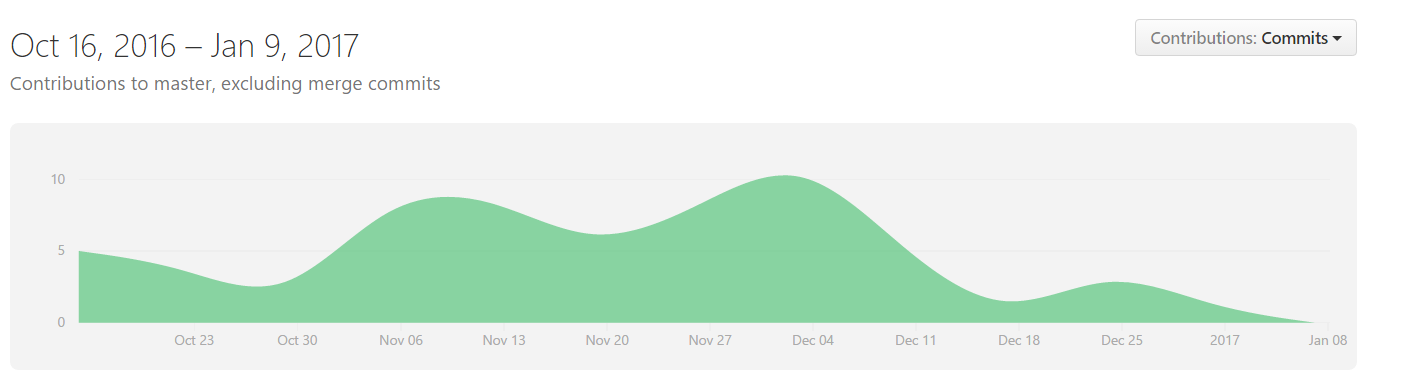
\includegraphics[width=.9\textwidth]{img/commits}
\caption{Distribución de los commits a lo largo del tiempo.}
\label{fig:Commits}
\end{figure}

En este segundo gráfico \ref{fig:punch_card} podemos observar las horas más fructíferas de trabajo. Dado que por las mañana trabajaba el número de commits es significativamente más bajo, en cambio por las tardes en torno las 19:00 es donde vemos un mayor número.

\begin{figure}
\centering
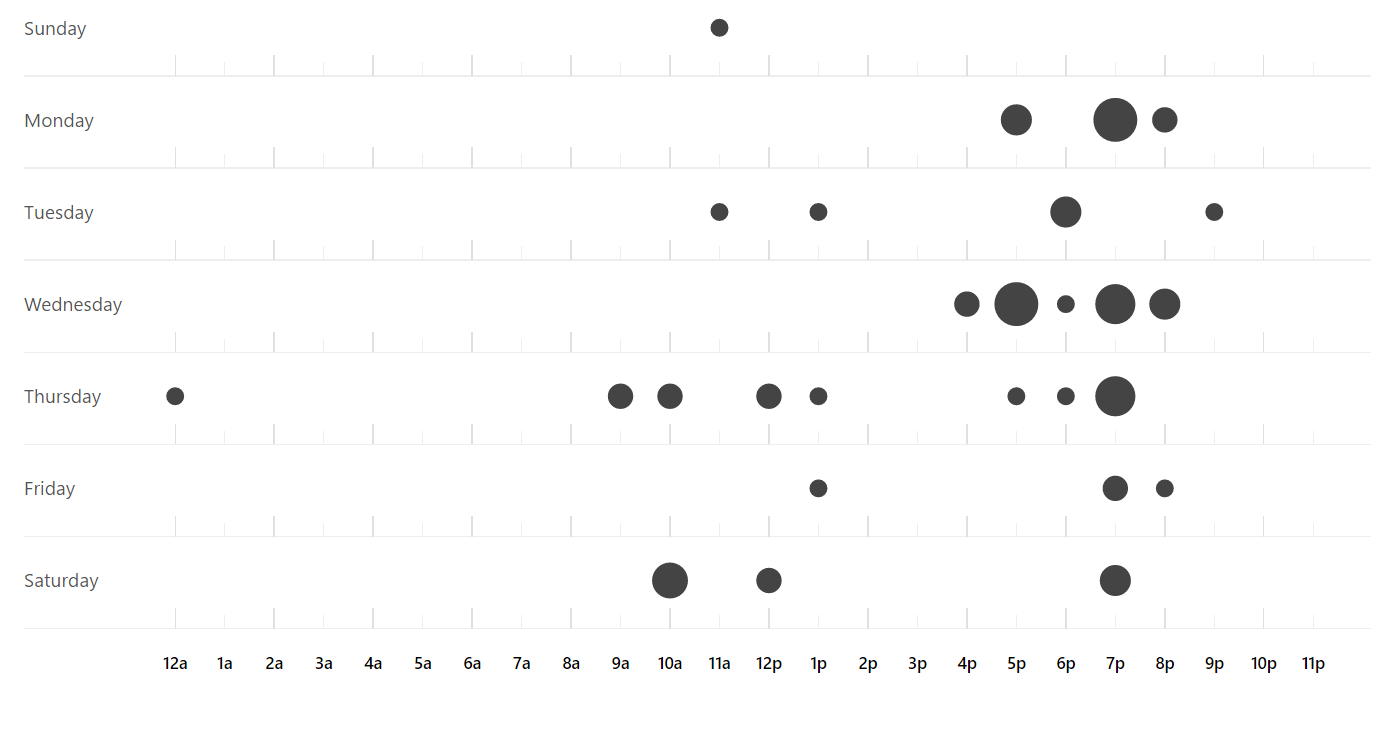
\includegraphics[width=.9\textwidth]{img/punch_card}
\caption{Distribución de los commits en días y horas.}
\label{fig:punch_card}
\end{figure}
 



\section{Estudio de viabilidad}
En esta sección vamos a analizar si se puede apostar o no por este proyecto en un futuro, vamos a tener en cuenta diferentes puntos de vista, como la viabilidad económica y la legal. Sin duda ambos factores son determinantes para seguir con el proyecto o al menos para que podamos lucrarnos de ello.


\subsection{Viabilidad económica}
Vamos a ver una visión económica del coste que supondría realizar este proyecto, para un único trabajador durante 4 meses, trabajando 2 horas diarias.

Es necesario contratar a un trabajador con experiencia en Drupal y PHP, que tenga cierta soltura para trabajar con bases de datos, estimamos que el sueldo del trabajador será de 20\euro{} /hora netos, por lo que el 32,1\% de cotización a la Seguridad Social \cite{cotizacion_ss} le corresponde a la empresa.
Teniendo en cuenta 22 dias laborables al mes:

22 dias/mes * 2 horas/dia * 20\euro/hora = 880\euro/mes a pagar al trabajador.
Teniendo en cuenta el pago de la SS:
880*1.321=1168.42\euro{} al mes hay que invertir en el trabajador.

Esto supone que los 4 meses de duración del proyecto suponen 4649.92\euro{}.

Ahora hay que analizar el coste que supone el hardware y el software, como todas las herramientas utilizadas o tenían licencia GNU o una version gratuita suficiente, no ha sido necesario ningún coste en lo referente a software.
En cuanto al hardware, el equipo tiene como especificaciones: Intel Core i7, 8GB de RAM y un disco duro de 1TB, el precio aproximado del equipo es de 850\euro{}. El plazo de amortización es de 4 años.

\begin{itemize}
\item Gastos de amortización anuales: 212.5 \euro{}
\item Coste mensual: 212.5 / 12 = 17.71 \euro{}
\item Como el proyecto es de 4 meses el gasto de amortización es: 17.71\euro{} * 4 = 70.83\euro{}
\end{itemize}

Los gastos mensuales de Internet son de 50\euro{} mensuales, suponiendo 200\euro{} al final del proyecto.

Los costes totales ascienden a:
4649.92 + 70.83 + 200 = 4920.75 \euro{}

La viabilidad económica del proyecto una vez realizado, en un futuro podemos enfocarla de dos formas, ya que depende del uso del programa o de la venta a una empresa del mismo.
\begin{itemize}
\item Uso personal: Los beneficios y pérdidas que se han ido logrando, podemos observarlos en el balance general, lo normal es que cuanta más información posea la red neuronal, mejores resultados nos de.{Imagen}

\item Venta a empresas: Sin duda esta no es la finalidad del proyecto, es difícil que una casa de apuestas opte por un proyecto como este dado que hay servicios de multinacionales que nos ofrecen una mayor capacidad de computación que el nuestro. Este proyecto lo veo algo más destinado al pequeño consumidor que quiera consultar resultados y opciones de apuestas en un momento dado.

No obstante dado que la licencia utilizada en GNU/GPL no se han realizado cálculos de licencias u otras formas de generar dinero.
\end{itemize}

\subsection{Viabilidad legal}
En el aspecto legal la única técnica cuestionable es el web scraping. En cuánto a su uso, se considera ilegal si puede generar un riesgo de asociación o comporte un aprovechamiento indebido de la reputación o el esfuerzo ajeno, es decir, es desleal sin supone un obstáculo a la afirmación de esa empresa en el mercado. El Tribunal Supremo dicta que las técnicas de scraping constituyen una técnica legal si se cumplen determinadas condiciones y supuestos.[referencia]

En resumidas cuentas, no depende del scraping en sí mismo, sino del uso que se le dan a los datos extraídos con este mismo. Si el uso de estos datos resultan competencias desleal nos encontraremos ante un acto ilegal.

Las licencias de los programas utilizados tienen las siguientes licencias:
\begin{itemize}
\item \textbf{Drupal: } GPL v2 y GPL v3.
\item \textbf{VirtualBox: } Privativa y GPL.
\item \textbf{Ubuntu: } GPL y otras licencias libres.
\item \textbf{Apache: } Licencia Apache 2.0.
\item \textbf{MySQL: } GPL o uso comercial.
\item \textbf{PHP: } Licencia PHP.
\end{itemize}

Como vamos a nombrar copyleft, es necesario explicar brevemente de lo que trata. Consiste en permitir una libre distribución de copias y versiones modificadas, donde los derechos de autor persisten en las versiones modificadas\cite{wiki:copyleft}.

La licencia GNU GPL es la licencia más utilizada en cuanto a software libre. Tiene como propósito decir que el software es libre, pero se encuentra protegido mediante \textit{copyleft}, de apropiación externa\cite{wiki:gnu_gpl}.

La licencia de PHP es una licencia de software libre pero que no permite copyleft a diferencia de la GNU GPL. La licencia PHP no es compatible con la licencia GPL\cite{wiki:licencia_php}.

En cuanto a la licencia Apache, se trata también de una licencia de software libre permisiva, requiere la conservación de los derechos de autor pero no es copyleft \cite{wiki:licencia_apache}.

Una vez realizado este análisis de las licencias utilizadas, hemos decidido poner una licencia GNU GPL al  proyecto dado que queremos mantener los derechos de autor, además gracias al \textit{copyleft} mantenemos los derechos si se llevan a cabo nuevas versiones.

